% Source of CSWBMCM2639496_extended.pdf. Build in this folder with two runs of
%   xelatex -jobname=CSWBMCM2639496_extended main.tex
% (fonts: TeX Gyre Termes/Heros, STIX Two Math, Noto Serif CJK SC) and copy CSWBMCM2639496_extended.pdf to ../
\documentclass[a4paper,11pt]{article}
\usepackage{fontspec}
\setmainfont{TeX Gyre Termes}
\setsansfont{TeX Gyre Heros}
\newfontfamily\cjkfont{Noto Serif CJK SC}
\usepackage{amsmath}
\usepackage{unicode-math}
\setmathfont{STIXTwoMath-Regular.otf}
\usepackage[a4paper,top=2.5cm,bottom=2.4cm,left=2.6cm,right=2.6cm]{geometry}
\usepackage{graphicx,booktabs,array,threeparttable,pdfpages,fancyhdr,xurl}
\usepackage[font=small,labelsep=period,skip=4pt]{caption}
\usepackage[hidelinks,bookmarksnumbered=true,bookmarksopen=true]{hyperref}
\usepackage{titlesec}
\renewcommand{\floatpagefraction}{0.8}\renewcommand{\topfraction}{0.88}\renewcommand{\bottomfraction}{0.7}\renewcommand{\textfraction}{0.1}
\usepackage{etoolbox}\AtBeginEnvironment{thebibliography}{\small\linespread{1.05}\selectfont\setlength{\itemsep}{1pt}\setlength{\parskip}{0pt}}
\setlength{\emergencystretch}{3em}
\linespread{1.15}
\setlength{\parskip}{0.25em}
\titleformat{\section}{\large\bfseries}{E\arabic{section}}{0.8em}{}
\titleformat{\subsection}{\normalsize\bfseries}{E\arabic{section}.\arabic{subsection}}{0.6em}{}
\renewcommand{\thesection}{E\arabic{section}}
\renewcommand{\thefigure}{E\arabic{figure}}
\renewcommand{\thetable}{E\arabic{table}}
\renewcommand{\theequation}{E\arabic{equation}}
\setlength{\headheight}{15pt}\pagestyle{fancy}\fancyhf{}\renewcommand{\headrulewidth}{0.4pt}
\newcommand{\hd}[1]{\begin{tabular}[b]{@{}c@{}}#1\end{tabular}}
\newcommand{\exthead}[1]{\fancyhead[L]{\small #1}\fancyhead[R]{\small Part II\quad Post-competition extensions}\fancyfoot[C]{\small E-\thepage}}

\graphicspath{{../../figures/extension/}}
\hypersetup{pdftitle={From egocentric hand records to restocking decisions -- extended edition}}
\begin{document}
\thispagestyle{empty}
\begin{center}
{\Large\bfseries From Egocentric Hand Records to Restocking Decisions:\\[0.2em] Calibrated State Prediction, Re-observation and Reservation Scheduling}\\[0.7em]
{\large Extended edition --- note}
\end{center}
\vspace{0.8em}

This file has two parts. Part I is the paper submitted to Problem C of the 12th ShuWei Cup mathematical modeling challenge, autumn 2026 (39 pages), reproduced exactly as submitted. Part II, starting on page E-1, contains post-competition extensions written in November 2026.

The paper builds one chain from 69 egocentric demonstration records to restocking decisions: a structural state-space model of the hand with a Markov reliability chain (Problem 1), split-conformal calibration of a prediction ball and a re-observation rule (Problem 2), and a rollout scheduling policy with a hierarchical duration model, selected by a pool-level one-standard-error rule (Problem 3). Part II first records a portability fix and a clean-room rerun that reproduced all 78 judged result files exactly. E1 then replays the Problem 3 policies on 300 seeds that had never been used. The reversal between the validation and test pools turns out to be a property of the environments, not of the seeds, and one test environment explains most of it; the emulated pools on which the selection rule relied did not anticipate it. E2 asks whether the 90\,\% prediction ball of Problem 2 holds in an environment it has not seen. Under the submitted calibration, coverage in a new environment ranges from 0.76 to 0.995; online adaptive conformal inference keeps every environment at or above 0.86 while enlarging the mean radius by only 4\,\%.

Every number in Part II can be reproduced with the scripts in the \texttt{extension/} folder of the code repository; result files are in \texttt{results/extension/}. The official dataset is not redistributed.

\clearpage
\pdfbookmark[0]{Part I\quad Competition paper (as submitted)}{part1}
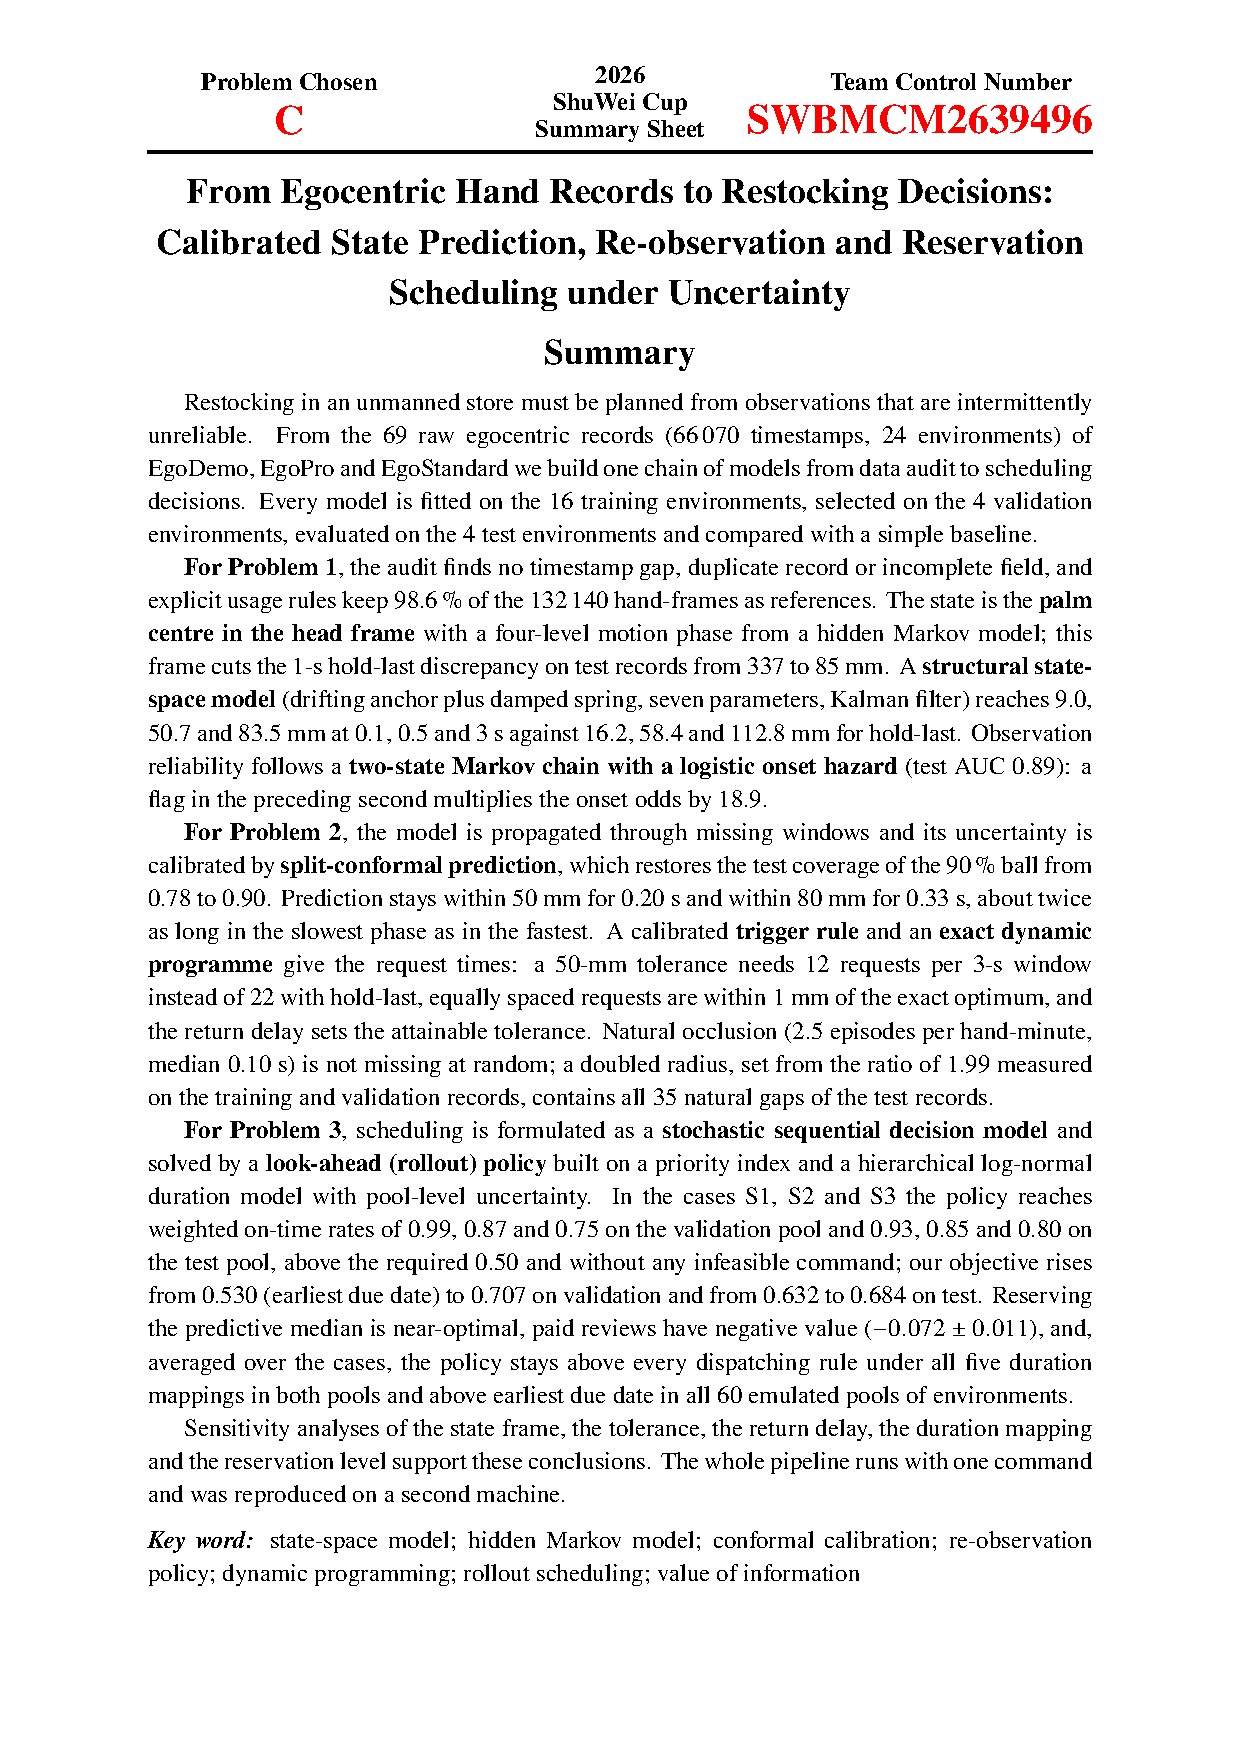
\includepdf[pages=-]{../CSWBMCM2639496.pdf}
\pdfbookmark[0]{Part II\quad Post-competition extensions}{part2}
\setcounter{page}{1}
\exthead{From egocentric hand records to restocking decisions}
\begin{center}{\Large\bfseries Part II\quad Post-competition extensions}\end{center}

Every model of the paper is fitted on 16 training environments, selected on 4 validation environments and evaluated on 4 test environments. Two of its conclusions rest on small evaluation samples that the contest could not enlarge. The choice of the Problem 3 scheduling policy was compared on 30 public validation seeds and 30 self-chosen test seeds, and the organisers score it on 30 undisclosed seeds. The 90\,\% guarantee of the Problem 2 prediction ball was established for windows pooled over environments, whereas the operational question is whether it holds in a store the model has never seen. Part II addresses both, after a reproduction check.

\paragraph{Reproduction and a portability fix.} The command \texttt{python code/run\_all.py --procs 2} reruns the whole pipeline from the official data in 16--18 minutes on two cores. In the documented layout, with the support folder next to the official data folder, two figure and table programs failed because they searched for the task files only inside the package instead of using the task-folder resolution of the shared module. Both now use that resolution; no computation changed. With this fix a clean rerun reproduced all 78 judged result files cell by cell, 964\,058 numeric cells with a largest relative difference of 0.0; four further files record run times and are listed but not judged. This rerun used the same Linux library versions as the original run; the cross-platform check is the Windows rerun recorded with the submission, with a largest relative difference of $3\times10^{-5}$.

\section{What does a 30-seed evaluation of Problem 3 tell?}

\subsection{Design}
The submission's two seed pools disagree. On the 30 validation seeds the policies with prefix-feature duration priors beat the selected policy \texttt{FROZEN}, which uses a family-level prior; on the 30 test seeds \texttt{FROZEN} wins. Thirty seeds cannot separate an effect of the environments from seed noise, so the six policies were replayed on 300 seeds that had never been used (2026130000--2026130299) with the submission's own command. These are \texttt{FROZEN}, the static and the on-line-learning prefix-feature priors, the model-averaged prior, the earliest-due-date (EDD) baseline and the clairvoyant benchmark, which knows all durations. The replays cover 300 seeds, 3 cases and the 5 duration mappings prescribed by the problem statement, that is, 4\,500 trials per policy and pool and 54\,000 trials in total, without a single invalid action. Replays are deterministic and do not depend on which policies share a batch: \texttt{FROZEN} replayed alone on the public seeds reproduces the submitted trials exactly. Seeds are the independent unit, because all policies see the same jobs for a given seed, so policy differences are paired by seed. The numbers below refer to the nominal duration mapping, on which the headline objective $U$ of Part I, the selection rule and the service floor are defined; averages over all five mappings give the same signs. The sampling distribution of a 30-seed evaluation is obtained from 5\,000 random 30-seed subsets of the 300 seeds.

\subsection{Results}

\begin{table}[htbp]\centering\small\setlength{\tabcolsep}{4pt}
\caption{Objective $U$ under the nominal mapping: mean over 300 new seeds with 95\,\% confidence interval, and the value reported in the submission on 30 seeds.}\label{tab:sw-e1}
\begin{tabular}{lcccc}\toprule
 & \multicolumn{2}{c}{Validation pool} & \multicolumn{2}{c}{Test pool}\\\cmidrule(lr){2-3}\cmidrule(lr){4-5}
Policy & 300 seeds [95\,\% CI] & 30 seeds & 300 seeds [95\,\% CI] & 30 seeds\\\midrule
\texttt{FROZEN} (family prior) & 0.701 [0.689, 0.713] & 0.707 & 0.731 [0.690, 0.772] & 0.684\\
Prefix-feature prior & 0.731 [0.720, 0.741] & 0.739 & 0.681 [0.645, 0.716] & 0.628\\
Prefix-feature prior, on-line learning & 0.724 [0.711, 0.737] & 0.739 & 0.670 [0.632, 0.709] & 0.614\\
Model-averaged prior & 0.725 [0.714, 0.737] & 0.736 & 0.724 [0.688, 0.759] & 0.679\\
EDD baseline & 0.527 [0.507, 0.546] & 0.530 & 0.698 [0.654, 0.741] & 0.632\\
Clairvoyant (durations known) & 0.881 [0.874, 0.889] & 0.889 & 0.920 [0.910, 0.931] & 0.904\\\bottomrule
\end{tabular}
\end{table}

\begin{table}[htbp]\centering\small\setlength{\tabcolsep}{4pt}
\caption{Paired difference \texttt{FROZEN} minus alternative (nominal mapping): mean over 300 seeds with 95\,\% confidence interval, share of random 30-seed subsets on which \texttt{FROZEN} is ahead, and the submitted 30-seed difference.}\label{tab:sw-e1b}
\begin{tabular}{llccc}\toprule
Pool & Alternative & 300 seeds [95\,\% CI] & \texttt{FROZEN} ahead (30 seeds) & Submitted\\\midrule
Validation & Prefix-feature prior & $-0.030$ [$-0.036$, $-0.024$] & 0.02\,\% & $-0.032$\\
 & Prefix-feature, on-line & $-0.023$ [$-0.030$, $-0.016$] & 1.1\,\% & $-0.032$\\
 & Model-averaged prior & $-0.025$ [$-0.030$, $-0.019$] & 0.3\,\% & $-0.029$\\
 & EDD baseline & $+0.174$ [$+0.163$, $+0.185$] & 100\,\% & $+0.177$\\\midrule
Test & Prefix-feature prior & $+0.051$ [$+0.041$, $+0.061$] & 99.8\,\% & $+0.056$\\
 & Prefix-feature, on-line & $+0.061$ [$+0.051$, $+0.071$] & 100\,\% & $+0.070$\\
 & Model-averaged prior & $+0.008$ [$-0.004$, $+0.019$] & 69.9\,\% & $+0.005$\\
 & EDD baseline & $+0.034$ [$+0.025$, $+0.043$] & 99.6\,\% & $+0.052$\\\bottomrule
\end{tabular}
\end{table}

\begin{figure}[htbp]\centering
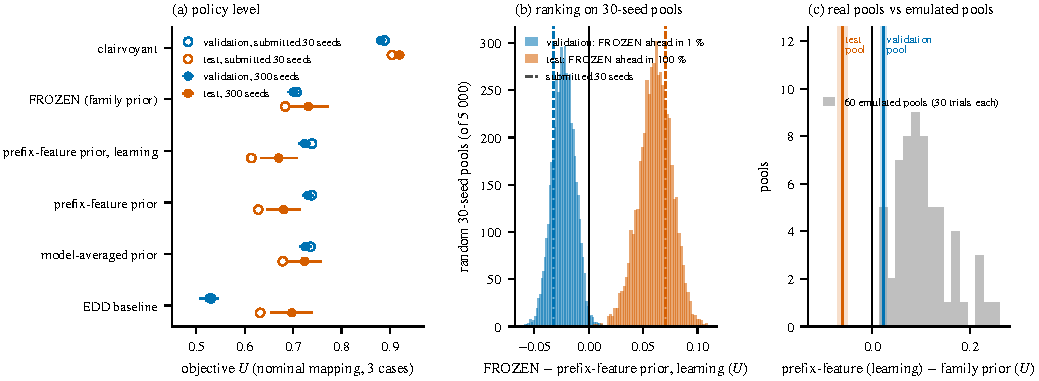
\includegraphics[width=\textwidth]{figE1_seed_replication.pdf}
\caption{Problem 3 policies on 300 new seeds (nominal mapping). (a) Objective $U$ per policy: mean over 300 seeds with 95\,\% confidence interval (filled markers) and the submitted 30-seed value (open markers), for the validation and test pools. (b) Paired difference \texttt{FROZEN} minus the on-line-learning prefix-feature prior over 5\,000 random 30-seed subsets; dashed lines mark the submitted 30-seed values. (c) The same comparison, with the opposite sign, on the 60 emulated pools used by the selection rule (histogram) and on the two real pools (vertical lines).}\label{fig:sw-e1}
\end{figure}

The reversal is a property of the environment pools, not of the seeds (Tables~\ref{tab:sw-e1} and~\ref{tab:sw-e1b}, Figure~\ref{fig:sw-e1}). Paired over 300 seeds, \texttt{FROZEN} trails the prefix-feature prior by 0.030 [0.024, 0.036] on the validation pool and leads it by 0.051 [0.041, 0.061] on the test pool. The swing of 0.081 has a seed-noise standard error of 0.006. On random 30-seed subsets of the same environments the sign of this comparison almost never changes: \texttt{FROZEN} is ahead on 0.02\,\% of validation subsets and on 99.8\,\% of test subsets. The standard deviation of the paired difference over 30 seeds is 0.010 on the validation pool and 0.016 on the test pool, so the difference between the two environment pools is 5.2 to 8.5 times the 30-seed noise. This confirms the premise of the pool-level selection rule of Part I, namely that variation between pools of environments, not trial noise, sets the uncertainty of a choice.

One test environment explains most of the reversal. The submission's held-out duration results already show that the 0.2-s prefix features lower the error of the log-duration prediction on the validation environments (0.43 against 0.56 for the family prior) but raise it on the test environments (0.52 against 0.37). The increase is concentrated in \texttt{logistics\_x\_courier\_station\_0041}, which contributes 21 of the 62 test units: there the error is 0.70 against 0.25, and the prefix model over-predicts durations by a factor of about 1.7 in geometric mean. Replaying the priors on the same 300 seeds with that environment removed from the test pool moves the gap of the static prefix-feature prior relative to the family prior from $-0.051$ to $+0.001$ [$-0.009$, $0.011$], and that of the learning variant from $-0.061$ to $-0.013$ [$-0.023$, $-0.003$]. Because the policies never read which pool a job comes from, removing the environment changes only the mix of jobs and not the policies. Across the trials of the full test pool the gap also falls with the share of jobs drawn from that environment, with a slope of $-0.14$ [$-0.25$, $-0.03$] per unit share for the static prior.

The emulated pools did not predict the test outcome. On the 60 emulated pools of training environments that the selection rule used, the prefix-feature priors beat the family prior on average, by 0.058 for the static and 0.105 for the learning variant, and the learning variant wins in all 60 pools. The validation pool lies at the median of this distribution for the static prior and at its 5th percentile for the learning variant, whereas the test pool lies below 59 of the 60 emulated pools for the static prior and below all 60 for the learning variant. The rule chose the family prior because it is the simplest configuration within one pool-level standard deviation of the best\cite{esl}, and on this test pool the choice paid off; the emulation itself pointed the other way. In hindsight the model-averaged prior is the most robust configuration: it is within 0.008 of the best prior on both real pools, a largest regret of 0.008 against 0.030 for \texttt{FROZEN} and 0.051--0.061 for the prefix-feature priors (over all five mappings, 0.019 against 0.025 for \texttt{FROZEN}). This suggests that averaging the two duration experts is the safer design when a test environment may break the prefix features.

The submitted levels were also affected by an unfavourable draw of test seeds. Every policy's submitted test mean lies at the 17th to 23rd percentile of the distribution of random 30-seed means, so the submitted test levels understate the 300-seed levels by 0.02 for the clairvoyant benchmark, about 0.05 for \texttt{FROZEN} and the learnt priors, and 0.07 for EDD. The gain of \texttt{FROZEN} over EDD on the test pool is $+0.034$ [0.025, 0.043] rather than the submitted $+0.052$, and \texttt{FROZEN} is ahead on 99.6\,\% of random 30-seed subsets; on the validation pool the gain is $+0.174$ [0.163, 0.185]. The distance to the clairvoyant benchmark is 0.181 on the validation pool and 0.189 on the test pool. The weighted on-time rate of \texttt{FROZEN} is 0.98, 0.85 and 0.75 in cases S1, S2 and S3 of the validation pool and 0.95, 0.87 and 0.84 in the test pool. None of the 5\,000 random 30-seed subsets falls below the service floor of 0.50; the 1\,\% quantile in the weakest case (S3, validation) is 0.70. The EDD baseline, by contrast, would fail the floor in case S3 of the validation pool on 23\,\% of 30-seed subsets.

\subsection{Protocol note and boundaries}
The pool-level selection rule was adopted after the test pool had been inspected under an earlier trial-level one-standard-error rule, which selects a prefix-feature prior. The submitted test comparison is therefore not a blind confirmation. Fresh seeds remove seed noise but not this earlier look at the test environments, so the evidence supports the statement that the family prior is better on this test pool because of one environment, and not the statement that the pool-level rule selects well in general. Only six policies were replayed, and the ablations and reservation variants of the submission were not. The emulated pools are resamples of training environments and cannot represent environment types that are absent from training. The objective $U$ and the duration mappings are the submission's own constructions on top of the official scoring rules.

\section{Does the 90\,\% prediction ball of Problem 2 hold in a new environment?}

\subsection{Design}
Problem 2 calibrates the radius of the prediction ball by split-conformal quantiles of the normalised prediction error\cite{vovk2005,lei2018}, pooling every window of the four validation environments, and reports a coverage of 0.90 pooled over the test windows. This marginal guarantee treats windows as exchangeable. Windows from one environment, however, share an operator, a layout and a mix of tasks, so the operational question is coverage in a new environment. E2 uses the eight environments that played no part in fitting the state model (2\,365 prediction onsets), holds out one environment at a time and calibrates on the other seven by four rules. The first is the submission's rule, which pools windows. The second pools environments with equal weight per environment, by CDF pooling for two-layer hierarchical data\cite{dunn2023}. The third takes the largest of the seven per-environment quantiles, guarding against the worst calibration environment. The fourth starts from the windows-pooled rule and adapts it on line inside the new environment by adaptive conformal inference\cite{gibbs2021}: the miscoverage level moves with outcomes that are already known when the next prediction onset arrives, and the step size $\gamma$ is not tuned.

\subsection{Results}

\begin{table}[htbp]\centering\small\setlength{\tabcolsep}{4pt}
\caption{Coverage of the nominal 90\,\% prediction ball in a held-out environment (all horizons up to 3 s, eight environments, leave one environment out). Online adaptation starts from the windows-pooled rule.}\label{tab:sw-e2}
\begin{tabular}{lcccc}\toprule
Calibration rule & Mean coverage & Worst environment & Below 0.85 & Mean radius\\\midrule
Windows pooled (submission) & 0.910 & 0.764 & 1 of 8 & 125 mm\\
Environments pooled & 0.894 & 0.692 & 1 & 119 mm\\
Worst calibration environment & 0.956 & 0.848 & 1 & 160 mm\\
Online adaptation, $\gamma=0.01$ & 0.921 & 0.862 & 0 & 130 mm\\
Online adaptation, $\gamma=0.005$ & 0.919 & 0.825 & 1 & 128 mm\\
Online adaptation, $\gamma=0.02$ & 0.919 & 0.881 & 0 & 132 mm\\\bottomrule
\end{tabular}
\end{table}

\begin{figure}[htbp]\centering
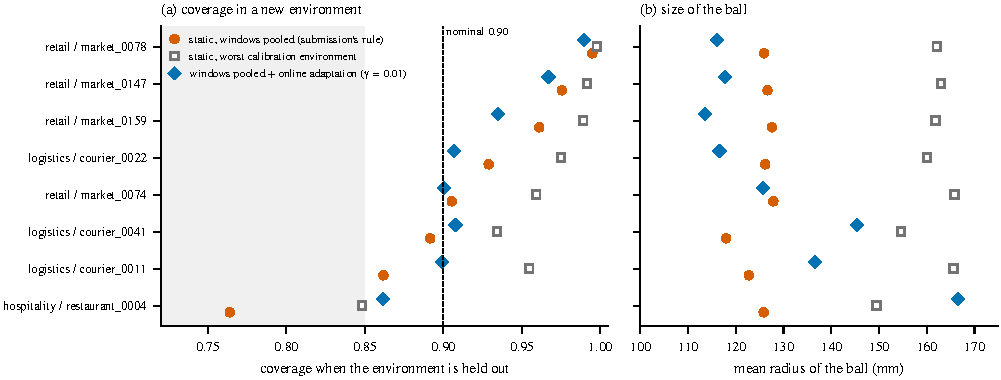
\includegraphics[width=0.94\textwidth]{figE2_environment_conformal.pdf}
\caption{The Problem 2 prediction ball in each held-out environment under three calibration rules: windows pooled (the submission's rule), the worst calibration environment, and windows pooled with online adaptation ($\gamma=0.01$). (a) Coverage of the nominal 90\,\% ball; the shaded region marks coverage below 0.85. (b) Mean radius of the ball.}\label{fig:sw-e2}
\end{figure}

One environment breaks the static guarantee (Table~\ref{tab:sw-e2}, Figure~\ref{fig:sw-e2}). Under the submission's rule, coverage in a held-out environment ranges from 0.76 to 0.995. The low end is the only hospitality environment, \texttt{hospitality\_x\_restaurant\_0004}, where coverage at the 3-s horizon is 0.76. On the four test environments the frozen validation calibration gives 0.874--0.996, which is consistent with this picture.

Static corrections do not help enough. Weighting environments equally lowers the radius, because the small retail environments are easy, and makes the worst case worse (0.69). Guarding against the worst calibration environment raises the restaurant to 0.85, but at the price of a ball that is 28\,\% larger in every environment. Adapting inside the new environment does help. With $\gamma=0.01$ every environment stays at or above 0.86. The restaurant rises from 0.76 to 0.86 as its ball grows from 126 to 167 mm, while easy environments receive smaller balls, for example 128 to 114 mm in \texttt{retail\_x\_supermarket\_0159}, and the mean radius rises by only 4\,\%. The adapted level occasionally exceeds 1 and is then clipped to the largest calibration score, for 0.7\,\% of predictions in the restaurant and 4.7\,\% in \texttt{logistics\_x\_courier\_station\_0041} at $\gamma=0.01$. At $\gamma=0.02$ clipping reaches 14--15\,\% in those two environments, and the guarantee then rests increasingly on the largest calibration score rather than on adaptation, which is why $\gamma=0.01$ is the sensible default.

For Problem 2 this matters directly, because the re-observation trigger fires when the calibrated ball exceeds the tolerance. In an environment like the restaurant the static calibration understates the ball at long horizons, so the trigger fires too late; online adaptation corrects this at almost no cost elsewhere.

\subsection{Conclusions and limits}

Both studies replace a statement about a fixed sample by a statement about the population the decision will face. For Problem 3, the 300-seed replay shows that the submitted ranking of policies is stable with respect to seeds but not with respect to environments, that a single environment carries the test-pool advantage of the selected policy, and that a model-averaged duration prior would have been the most robust choice across both pools. For Problem 2, the windows-pooled calibration delivers its nominal coverage on average but not in every environment, and online adaptive conformal inference closes the gap with a 4\,\% larger mean radius. The environment-level study is limited to eight environments of three types. The adaptation uses outcomes with their true delay of up to 3 s, but it treats the records of one environment as a single sequence, and the step size was fixed in advance rather than validated across environments.

\begin{thebibliography}{9}
\bibitem{esl} T. Hastie, R. Tibshirani, J. Friedman. \emph{The Elements of Statistical Learning}, 2nd edition. Springer, 2009.
\bibitem{vovk2005} V. Vovk, A. Gammerman, G. Shafer. \emph{Algorithmic Learning in a Random World}. Springer, 2005.
\bibitem{lei2018} J. Lei, M. G'Sell, A. Rinaldo, R. J. Tibshirani, L. Wasserman. Distribution-free predictive inference for regression. \emph{Journal of the American Statistical Association}, 113(523): 1094--1111, 2018. doi:10.1080/01621459.2017.1307116.
\bibitem{dunn2023} R. Dunn, L. Wasserman, A. Ramdas. Distribution-free prediction sets for two-layer hierarchical models. \emph{Journal of the American Statistical Association}, 118(544): 2491--2502, 2023. doi:10.1080/01621459.2022.2060112.
\bibitem{gibbs2021} I. Gibbs, E. Candès. Adaptive conformal inference under distribution shift. In \emph{Advances in Neural Information Processing Systems 34 (NeurIPS 2021)}, 2021.
\end{thebibliography}
\end{document}
